\documentclass{beamer}
\usetheme{Warsaw}
\usepackage{tikz}
\usetikzlibrary{positioning,shapes,arrows,overlay-beamer-styles}

\title{Beamer Overlay Techniques Demo}
\subtitle{Interactive Examples}
\author{LaTeX Overlay Guide}
\date{\today}

\begin{document}

\begin{frame}
    \titlepage
\end{frame}

\begin{frame}{Table of Contents}
    \tableofcontents
\end{frame}

\section{Basic Overlays}

\begin{frame}{Basic Pause Command}
    \begin{itemize}
        \item First point
        \pause
        \item Second point appears after pause
        \pause
        \item Third point appears last
    \end{itemize}
\end{frame}

\begin{frame}{Using \textbackslash only}
    \only<1>{This text appears only on slide 1}
    \only<2>{This text replaces it on slide 2}
    \only<3>{And this appears on slide 3}
    \only<4->{This stays from slide 4 onwards}
\end{frame}

\begin{frame}{Using \textbackslash uncover}
    \begin{block}{Space is Reserved}
        \uncover<1->{Always visible}
        
        \uncover<2->{Appears on slide 2 (space was reserved)}
        
        \uncover<3->{Appears on slide 3}
        
        \uncover<4>{Only on slide 4}
    \end{block}
\end{frame}

\begin{frame}{Using \textbackslash visible and \textbackslash invisible}
    \begin{columns}
        \column{0.5\textwidth}
        \textbf{Visible Demo:}
        \begin{itemize}
            \item \visible<1->{Always visible}
            \item \visible<2->{From slide 2}
            \item \visible<3>{Only on slide 3}
        \end{itemize}
        
        \column{0.5\textwidth}
        \textbf{Invisible Demo:}
        \begin{itemize}
            \item \invisible<2>{Hidden on slide 2}
            \item \invisible<3>{Hidden on slide 3}
            \item \invisible<1>{Hidden on slide 1}
        \end{itemize}
    \end{columns}
\end{frame}

\begin{frame}{Using \textbackslash alt}
    \begin{center}
        \Large
        \alt<1>{Welcome to Slide 1}{
        \alt<2>{Now on Slide 2}{
        \alt<3>{This is Slide 3}{
        Final Slide}}}
    \end{center}
    
    \vspace{1cm}
    
    \alt<2>{\color{red}Red on slide 2}{\color{blue}Blue on other slides}
\end{frame}

\section{Advanced Overlays}

\begin{frame}{Dynamic Highlighting with \textbackslash alert}
    \begin{theorem}
        The sum \alert<2>{$a + b$} equals \alert<3>{$c$} when 
        \alert<4>{$a = c - b$}.
    \end{theorem}
    
    \begin{itemize}
        \item<2-> We start with the sum
        \item<3-> We know the result
        \item<4-> We can derive the relationship
    \end{itemize}
\end{frame}

\begin{frame}{Automatic Incremental Lists}
    \begin{columns}
        \column{0.5\textwidth}
        \begin{block}{Manual}
            \begin{itemize}
                \item<1-> First
                \item<2-> Second
                \item<3-> Third
            \end{itemize}
        \end{block}
        
        \column{0.5\textwidth}
        \begin{block}{Automatic}
            \begin{itemize}[<+->]
                \item First
                \item Second
                \item Third
            \end{itemize}
        \end{block}
    \end{columns}
\end{frame}

\begin{frame}{Alert on Appearance}
    \begin{enumerate}[<+-| alert@+>]
        \item First item (highlighted when appearing)
        \item Second item (highlighted when appearing)
        \item Third item (highlighted when appearing)
        \item Fourth item (highlighted when appearing)
    \end{enumerate}
\end{frame}

\section{TikZ Integration}

\begin{frame}{TikZ with Overlays}
    \begin{center}
    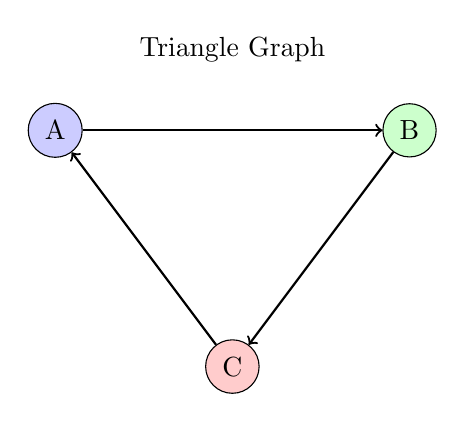
\begin{tikzpicture}[scale=1.5]
        % Nodes
        \node<1->[circle,draw,fill=blue!20] (A) at (0,0) {A};
        \node<2->[circle,draw,fill=green!20] (B) at (3,0) {B};
        \node<3->[circle,draw,fill=red!20] (C) at (1.5,-2) {C};
        
        % Edges
        \draw<4->[thick,->] (A) -- (B);
        \draw<5->[thick,->] (B) -- (C);
        \draw<6->[thick,->] (C) -- (A);
        
        % Label
        \node<7->[above] at (1.5,0.5) {Triangle Graph};
    \end{tikzpicture}
    \end{center}
\end{frame}

\begin{frame}{TikZ Visible On Style}
    \begin{center}
    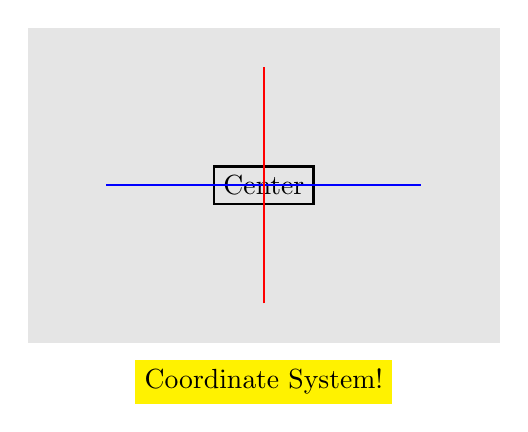
\begin{tikzpicture}
        % Background that's always visible
        \fill[visible on=<1->,gray!20] (-3,-2) rectangle (3,2);
        
        % Elements appearing in sequence
        \node[visible on=<2->,draw,thick] at (0,0) {Center};
        \draw[visible on=<3->,thick,blue] (-2,0) -- (2,0);
        \draw[visible on=<4->,thick,red] (0,-1.5) -- (0,1.5);
        
        % Temporary highlight
        \node[visible on=<5>,fill=yellow] at (0,-2.5) {Coordinate System!};
    \end{tikzpicture}
    \end{center}
\end{frame}

\section{Temporal Effects}

\begin{frame}{Using \textbackslash temporal}
    \begin{center}
    \temporal<2-4>
        {\Large Before activation}
        {\Huge\color{red}\textbf{ACTIVE!}}
        {\large\color{gray}After activation}
    \end{center}
    
    \vspace{1cm}
    
    \begin{itemize}
        \item<1-> Watch the text above
        \item<2-> It's now active
        \item<4-> Active phase ending...
        \item<5-> Back to inactive state
    \end{itemize}
\end{frame}

\begin{frame}{Complex Temporal Example}
    \begin{columns}
        \column{0.5\textwidth}
        \temporal<2-3>
            {\includegraphics[width=\textwidth]{example-image-a}}
            {\includegraphics[width=\textwidth]{example-image-b}}
            {\includegraphics[width=\textwidth]{example-image-c}}
            
        \column{0.5\textwidth}
        \temporal<2-3>
            {Initial state image}
            {\color{red}\textbf{Processing...}}
            {\color{green}Complete!}
    \end{columns}
\end{frame}

\section{Practical Examples}

\begin{frame}{Code Reveal}
    \begin{block}{Python Function}
        \begin{semiverbatim}
\uncover<1->{def fibonacci(n):}
\uncover<2->{    if n <= 1:}
\uncover<3->{        return n}
\uncover<4->{    else:}
\uncover<5->{        return fibonacci(n-1) + fibonacci(n-2)}
        \end{semiverbatim}
    \end{block}
    
    \begin{itemize}
        \item<2-> Base case check
        \item<3-> Return for base cases
        \item<5-> Recursive calls
    \end{itemize}
\end{frame}

\begin{frame}{Mathematical Proof}
    \begin{theorem}
        $\sum_{i=1}^{n} i = \frac{n(n+1)}{2}$
    \end{theorem}
    
    \begin{proof}
        \only<1>{We'll prove this by induction.}
        
        \only<2>{Base case: $n=1$
        $$\sum_{i=1}^{1} i = 1 = \frac{1(1+1)}{2} = 1 \checkmark$$}
        
        \only<3>{Inductive step: Assume true for $n=k$
        $$\sum_{i=1}^{k} i = \frac{k(k+1)}{2}$$}
        
        \only<4>{Show true for $n=k+1$:
        \begin{align}
        \sum_{i=1}^{k+1} i &= \sum_{i=1}^{k} i + (k+1)\\
        &= \frac{k(k+1)}{2} + (k+1)\\
        &= \frac{k(k+1) + 2(k+1)}{2}\\
        &= \frac{(k+1)(k+2)}{2} \checkmark
        \end{align}}
    \end{proof}
\end{frame}

\section{Handout Mode}

\begin{frame}{Mode-Specific Content}
    \only<beamer>{
        \begin{block}{Presentation Mode}
            This content only appears in presentation mode.
            \begin{itemize}
                \item<2-> Interactive elements
                \item<3-> Animations
                \item<4-> Step-by-step reveals
            \end{itemize}
        \end{block}
    }
    
    \only<handout>{
        \begin{block}{Handout Mode}
            This content only appears in handout mode.
            \begin{itemize}
                \item All content visible at once
                \item Suitable for printing
                \item No animations
            \end{itemize}
        \end{block}
    }
    
    \uncover<beamer:2-|handout:1>{
        This appears on slide 2+ in presentation, always in handout.
    }
\end{frame}

\section{Summary}

\begin{frame}{Summary of Overlay Commands}
    \begin{description}[<+->]
        \item[\textbackslash pause] Simple sequential reveal
        \item[\textbackslash only] Content replacement
        \item[\textbackslash uncover] Space-preserving reveal
        \item[\textbackslash alert] Dynamic highlighting
        \item[\textbackslash temporal] Three-state transitions
        \item[<+->] Automatic incrementing
    \end{description}
\end{frame}

\begin{frame}{Best Practices}
    \begin{columns}[t]
        \column{0.5\textwidth}
        \begin{block}{Do}
            \begin{itemize}[<+->]
                \item Use overlays purposefully
                \item Keep animations smooth
                \item Test in presentation mode
                \item Provide handout version
            \end{itemize}
        \end{block}
        
        \column{0.5\textwidth}
        \begin{block}{Don't}
            \begin{itemize}[<+->]
                \item Overuse animations
                \item Make content too complex
                \item Forget about timing
                \item Ignore accessibility
            \end{itemize}
        \end{block}
    \end{columns}
\end{frame}

\begin{frame}
    \begin{center}
        \Huge Thank You!
        
        \vspace{1cm}
        
        \large
        \temporal<2>
            {Questions?}
            {\color{red}Questions?}
            {See the comprehensive guide for more details}
    \end{center}
\end{frame}

\end{document}